\documentclass[11pt]{article}
\usepackage{amsmath}

\usepackage{amstext}

\usepackage{amsthm}
\usepackage{color, fullpage, hyperref}
\usepackage{amssymb}
\usepackage{mathtools}
\usepackage{commath}

\usepackage[table]{xcolor}
\usepackage{makecell}

\usepackage{graphicx}
\usepackage{tikz, pgfplots, hf-tikz}
\pgfplotsset{compat=1.17}
\allowdisplaybreaks
\renewcommand\qedsymbol{$\blacksquare$}
\usepackage{tcolorbox}
\tcbuselibrary{theorems}
\tcbuselibrary{fitting}
\usepackage{empheq}

\usepackage[margin=0.5in]{geometry}
\usepackage{fancyvrb}


\title{CSCB07 Lecture 10-12}
\author{Vinesh Benny}

\begin{document}
\section{Introduction to Android}
\begin{itemize}
	\item Android
		\begin{itemize}
			\item Android is a platform comprising of three components
				\begin{itemize}
					\item An operating system
					\item A framework for developing applications
					\item Devices that run the Android operating system and the applications created
					for it
				\end{itemize}
			\item Android SDK
				\begin{itemize}
					\item A collection of libraries and tools that are needed for developing Android applications
				\end{itemize}
			\item Android Studio
				\begin{itemize}
					\item IDE for Android application development
				\end{itemize}
		\end{itemize}

	\item Android App Basics
		\begin{itemize}
			\item An Android app is a collection of screens, and each screen is comprised of a layout and an activity
				\begin{itemize}
					\item Layout: describes the appearance of a screen (written in XML)
					\item Activity: responsible for managing user interaction with the screen (written in java)
				\end{itemize}
			\item Folder structure:
				\begin{itemize}
					\begin{minipage}[t]{0.15\textwidth}
						\item Manifest file
						\item Java file
					\end{minipage}
					\begin{minipage}[t]{0.3\textwidth}
						\item Resource files
						\item Gradle scripts
					\end{minipage}
				\end{itemize}
		\end{itemize}
	\item The Manifest file
		\begin{itemize}
			\item It defines the structure and metadata of an application, its components, and its requirements
			\item Stored in the root of its project hierarchy as an XML file
		\end{itemize}

	\item Resources and resource IDs
		\begin{itemize}
			\item Resources are maintained in sub-directories of the \Verb|app/res| directory
				\begin{itemize}
					\item \Verb|res/layout|
					\item \Verb|res/values|
					\item Etc.
				\end{itemize}
			\item A resource can be accessed in the code using its resource ID (e.g. \Verb|R.layout.activity_main|)
				\begin{itemize}
					\item Android uses \Verb|R.java| to keep track of the resources used within the app
				\end{itemize}
		\end{itemize}

	\item View
		\begin{itemize}
			\item Most GUI components are instances of the \textbf{View} class or one of its subclasses
				\begin{itemize}
					\item e.g. Button, EditText, ImageView, etc.
				\end{itemize}
				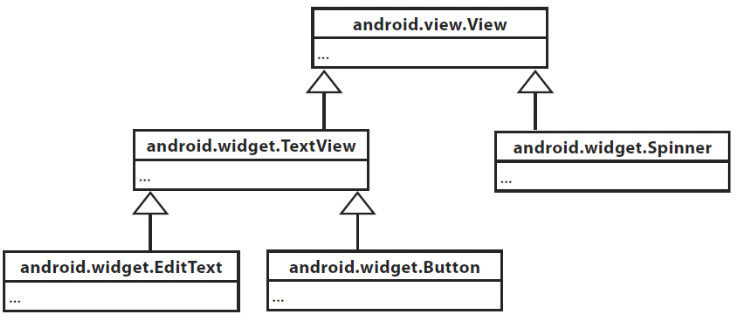
\includegraphics[scale=0.7]{View.png}
		\end{itemize}

	\newpage
	\item View Group
		\begin{itemize}
			\item A special type of view that can contain other views
			\item A layout is a type of view group\\
			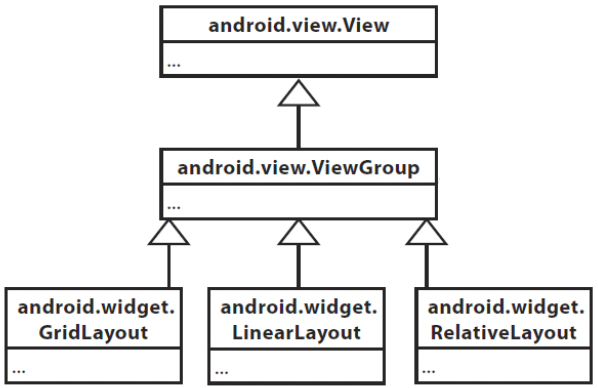
\includegraphics[scale=0.7]{ViewGroup.png}
		\end{itemize}

	\item Common GUI compnents
		\begin{itemize}
			\begin{minipage}[t]{0.15\textwidth}
				\item TextView
				\item EditText
				\item Button
			\end{minipage}
			\begin{minipage}[t]{0.15\textwidth}
				\item Switch
				\item Spinner
				\item Toast
			\end{minipage}
		\end{itemize}

	\item Intents
		\begin{itemize}
			\item An intent is an object that can be used to bind activities together at runtime
				\begin{itemize}
					\item If one activity wants to start a second activity, it does it by sending an intent to Android. Android will start the second activity and pass it the intent
				\end{itemize}
			\item Data can be passed between activities using intent extras
				\begin{itemize}
					\item e.g. \Verb|intent.putExtra("message", value);|
				\end{itemize}
		\end{itemize}
\end{itemize}

\newpage
\section{Android - Storing Data}
\begin{itemize}
	\item Data storage options
		\begin{itemize}
			\item File system
			\item Shared preferences
			\item Databases
				\begin{itemize}
					\item e.g. SQLite, Firebase Realtime Database
				\end{itemize}
		\end{itemize}

	\item File system
		\begin{itemize}
			\item Android’s file system consists of six main partitions
				\begin{itemize}
					\begin{minipage}[t]{0.15\textwidth}
						\item \Verb|/boot|
						\item \Verb|/system|
					\end{minipage}
					\begin{minipage}[t]{0.15\textwidth}
						\item \Verb|/recovery|
						\item \Verb|/data|
					\end{minipage}
					\begin{minipage}[t]{0.15\textwidth}
						\item \Verb|/cache|
						\item \Verb|/misc|
					\end{minipage}
				\end{itemize}
			\item Reading/writing data to a file on internal storage can be done using
				\begin{itemize}
					\begin{minipage}[t]{0.23\textwidth}
						\item \Verb|openFileInput()|
					\end{minipage}
					\begin{minipage}[t]{0.2\textwidth}
						\item \Verb|openFileOutput()|
					\end{minipage}
				\end{itemize}
		\end{itemize}

	\item Shared preferences
		\begin{itemize}
			\item Suitable for simple data that could be stored as key/value pairs
			\item A \textbf{SharedPreferences} object refers to a file containing key/value pairs and provides methods to read and write them
			\item Creating/accessing shared preference files can be done using:
				\begin{itemize}
					\begin{minipage}[t]{0.23\textwidth}
						\item \Verb|getPreferences()|
					\end{minipage}
					\begin{minipage}[t]{0.3\textwidth}
						\item \Verb|getSharedPreferences()|
					\end{minipage}
				\end{itemize}
		\end{itemize}

	\item SQLite
		\begin{itemize}
			\begin{minipage}[t]{0.22\textwidth}
				\item Relational database
				\item Serverless
			\end{minipage}
			\begin{minipage}[t]{0.22\textwidth}
				\item Zero-configuration
				\item File-based
			\end{minipage}
			\begin{minipage}[t]{0.15\textwidth}
				\item Widely used
			\end{minipage}
		\end{itemize}

	\item Firebase Realtime Database
		\begin{itemize}
			\item Cloud-hosted
			\item Employs data synchronization
				\begin{itemize}
					\item Every time data changes, all connected clients automatically receive updates
				\end{itemize}
			\item NoSQL
				\begin{itemize}
					\item Data is stored as JSON
				\end{itemize}
			\item The Firebase SDK provides many classes and methods to store and sync data. E.g.
				\begin{itemize}
					\begin{minipage}[t]{0.24\textwidth}
						\item \Verb|DatabaseReference|
						\item \Verb|DataSnapshot|
					\end{minipage}
					\begin{minipage}[t]{0.22\textwidth}
						\item \Verb|ValueEventListener|
					\end{minipage}
				\end{itemize}
		\end{itemize}

	\item JSON
		\begin{itemize}
			\item \textbf{J}ava\textbf{S}cript \textbf{O}bject \textbf{N}otation
			\item Language-independent
			\item Supported by many programming languages
			\item Uses readable text to represent data in the form of key/value pairs
			\item Example \begin{Verbatim}
{
	"name": "Alex”,
	"age”: 25,
	"address”: {
		"country”: "Canada”,
		"city”: "Toronto”
	}
}
			\end{Verbatim}

		\end{itemize}
\end{itemize}

\newpage
\section{Android  - Testing}
\begin{itemize}
	\item Model-View-Presenter
		\begin{itemize}
			\vspace{0.2cm}
			\begin{minipage}[b]{0.65\textwidth}
				\item An architectural design pattern that results in code that is easier to test
				\item It consists of three components:
				\begin{enumerate}
					\item Model (Data)
					\item View (UI)
					\item Presenter (Business logic)
				\end{enumerate}
			\end{minipage}
			\begin{minipage}[t]{0.2\textwidth}
				\vspace{-3.5cm}
				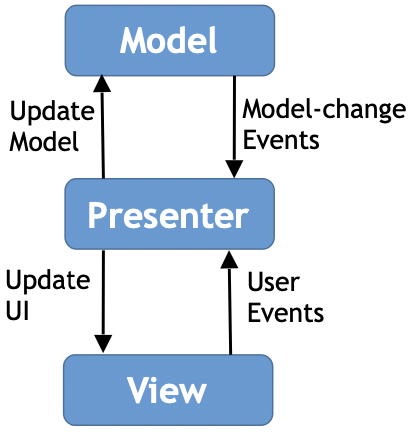
\includegraphics[scale=0.6]{MVP.png}
			\end{minipage}
		\end{itemize}

	\item Local and Instrumented Tests
		\begin{itemize}
				\vspace{0.2cm}
				\begin{minipage}[b]{0.5\textwidth}
					\item Local unit tests
					\begin{itemize}
						\item Run on the machine’s local JVM
						\item Do not depend on the Android framework
					\end{itemize}
				\item Instrumented tests
					\begin{itemize}
						\item Run on an actual device or an emulator
						\item Usually used for integration and UI tests
					\end{itemize}
				\end{minipage}
				\begin{minipage}[t]{0.4\textwidth}
					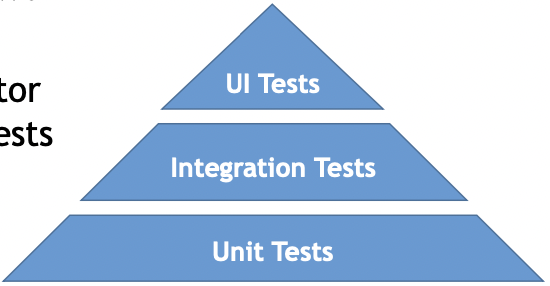
\includegraphics[scale=0.7]{LITests.png}
				\end{minipage}
		\end{itemize}

	\item Commonly used tools
		\begin{itemize}
			\item JUnit
				\begin{itemize}
					\item Writing unit tests
				\end{itemize}
			\item Mockito
				\begin{itemize}
					\item Creating dummy (mock) objects to facilitate testing a component in
					isolation
				\end{itemize}
			\item Roboelectric
				\begin{itemize}
					\item Running tests that involve the Android framework without an emulator or a device
				\end{itemize}
			\item Espresso
				\begin{itemize}
					\item Writing UI tests
				\end{itemize}
		\end{itemize}

	\item Mock Objects
		\begin{itemize}
			\item A mock is software component that is used to replace the “real” component during testing
			\item Mock objects could be used to:
				\begin{itemize}
					\item Represent components that have not yet been implemented
					\item Speed up testing
					\item Reduce the cost
					\item Avoid unrecoverable actions
					\item Etc.
				\end{itemize}
		\end{itemize}

	\item Mockito
		\begin{itemize}
			\item A mocking framework for Java
			\item Features include:
				\begin{itemize}
					\item Creating mocks
					\item Stubbing
					\item Verifying behavior
				\end{itemize}
		\end{itemize}
\end{itemize}
\end{document}